% !TeX spellcheck = sv_SE
%\documentclass[mathserif]{beamer}
\documentclass{beamer}
%\usepackage{default}

\usepackage[swedish]{babel}
\usepackage[T1]{fontenc}
\usepackage{lmodern}
\usepackage[utf8]{inputenc}

\usepackage{amsmath}
\usepackage{amssymb}
\usepackage{amsfonts}
\usepackage{amsthm}

\usepackage{icomma}

\usepackage{graphicx}

%\usepackage{enumitem}

\DeclareMathOperator{\sign}{sign}

\theoremstyle{definition}
\newtheorem{thm}{Sats}[section]
\newtheorem{lem}[thm]{Lemma}
\newtheorem{cor}[thm]{Korollarium}
\newtheorem{defi}{Definition}[section]
\newtheorem{ex}{Exempel}[section]
\theoremstyle{remark}
\newtheorem*{rem}{Observation}

\newtheorem*{reas}{Orsak}

\newcommand{\bfbeta}{{\boldsymbol{\beta}}}
\renewcommand\qedsymbol{$\blacksquare$}

\newcommand{\bfx}{\mathbf{x}}

\newcommand{\bfy}{\mathbf{y}}

\newcommand{\llangle}{\left\langle}
\newcommand{\rrangle}{\right\rangle}

\newcommand{\sephyp}{\{ \mathbf{x} : f\left(\mathbf{x}\right)=\inner{\bfx}{\bfbeta}_\mathcal{H} + \beta_0=0\}}

\newcommand{\entsephyp}{\{ \mathbf{x} : f\left(\mathbf{x}\right)=\mathbf{x}^\intercal \bfbeta + \beta_0=0,~y_if\left(\mathbf{x}_i\right)\geq0,~i=1,\dots,~N,~\left\|\bfbeta\right\|=1\}}

\newcommand{\inprod}[2]{\llangle \mathbf{#1}, \mathbf{#2}\rrangle}

\newcommand{\inner}[2]{\llangle #1, #2 \rrangle}

\newcommand{\hil}{\mathcal{H}}

\interfootnotelinepenalty=10000

\usetheme{Pittsburgh}
%\usetheme{EastLansing}

\usecolortheme{wolverine}
%\usecolortheme{fly}
%\usecolortheme{beetle}
%\usecolortheme{beaver}
%\usecolortheme{albatross}
%\setbeamerfont{title}{family=\rm}
\usefonttheme{serif}

%\setbeamercolor{title}{fg=red!80!black}
%\setbeamercolor{title}{fg=red!80!black,bg=red!20!white}
%\setbeamercolor*{palette primary}{fg=red, bg=red}
%\setbeamercolor{palette secondary}{fg=red, bg=red, use=blue, parent=blue}
%\setbeamercolor{palette sidebar primary}{fg=red, bg=red, use=blue, parent=blue}
%\setbeamercolor{title}{fg=white!95!black}
%\setbeamercolor{author}{fg=white!95!black}
%\setbeamercolor{date}{fg=white!95!black}
%\setbeamercolor{institute}{fg=white!95!black}
%\setbeamercolor{titlelike}{fg=white!95!black}
%\setbeamercolor{normal text}{fg=white!95!black}
%\setbeamercolor{background canvas}{bg=black!95!white}

\title{{\Huge Stödvektormaskiner}\\
	{\LARGE Linjära hyperplan i Hilbertrum}}
%	~\\
%	{\large Kandidatavhandling i matematik}}
%	{\large Fakulteten för naturvetenskaper och teknik}\\
%	{\large Åbo Akademi}}
\author{\Large Oscar Granlund}
\institute{{\large Kandidatavhandling i matematik}\\
	{\large Fakulteten för naturvetenskaper och teknik}\\
	{\large Åbo Akademi}}

\date{9 november 2018}
\begin{document}
%\maketitle
\begin{frame}
	\titlepage
\end{frame}

\begin{frame}
	\frametitle{Bakgrund}
	\framesubtitle{Klassificering med hjälp av hyperplan}
	Stödvektormaskinen utvecklades under den senare halvan av 1900-talet i huvudsak av den ryske statistikern/datavetaren Vladimir Vapnik.
	\begin{itemize}
		\item 	Tog sin början år 1963 med en \emph{linjär klassificerare} som endast gick att tillämpa på några problem.
		\item 	År 1992 presenterades en version som gick att tillämpa på alla problem.
	\end{itemize}
	Stödvektormaskinen går ut på att man skjuter in ett hyperplan mellan två klasser och använder hyperplanet för att klassificera nya observationer.
\end{frame}

\begin{frame}
	\frametitle{Bakgrund}
	\framesubtitle{En olinjär version}
	Parallellt med forskningen om stödvektormaskiner fann statistiker att en speciell typ av funktion, kärnor, kunde användas för att generalisera linjära algoritmer.
	\begin{itemize}
		\item	Kärnorna föreslogs redan år 1964 för att generalisera en annan typ av linjär klassificerare.
		\item 	De användes även för att studera till exempel spline-modeller.
		\item 	År 1992 tillämpades kärnor på den ursprungliga stödvektormaskinmetoden.
	\end{itemize}
	Snart därefter (1995) tillämpades kärnor på den mera generaliserade algoritmen som presenterades 1992. Resultatet är en (tidsmässigt och resultatmässigt) effektiv \emph{olinjär klassificerare} som ännu idag används.
\end{frame}

\begin{frame}
	\frametitle{Konvex optimering}
	\framesubtitle{Kvadratiska optimerignsproblem}
	De flesta av algoritmerna inom statistik och maskininlärning går att skriva om som konvexa optimeringsproblem.
	Ett optimeringsproblem är kvadratiskt och konvext om det går att skriva om på formen
	\begin{equation*}
	\begin{aligned}
	\operatornamewithlimits{min}_\bfx& & &\frac{1}{2}\bfx^\intercal\mathbf{P}\bfx+\mathbf{q}^\intercal\bfx + r\\
	\text{så att}& & &g_i(\bfx)\leq0,\quad i=1,~\dots,~n\\
	& & &h_i(\bfx)=0,\quad i=1,~\dots,~m,\\
	\end{aligned}
	\end{equation*}
	där $\mathbf{P}$ är en positivt semidefinit matris, $g_i(\bfx)$ är högst en kvadratisk funktion och alla krav $g_i$ och $h_i$ är satisfierbara samtidigt.
\end{frame}

\begin{frame}
	\frametitle{Konvex optimering}
	\framesubtitle{Lagrangefunktioner}
	Ett konvext optimeringsproblem med olikhetskrav och likhetskrav kan lösas  med hjälp av Lagrangemultiplikatorer.
	För ett kvadratiskt optimeringsproblem blir den primala Lagrangefunktionen
	\begin{equation*}
		L_P=f(\bfx) + \sum_{i=1}^{n}\lambda_ig_i(\bfx)+\sum_{i=1}^{m}v_ih_i(\bfx)
	\end{equation*}
	där $f(\bfx)$ är objektfunktionen och $g_i,~h_i$ är kraven.
	Den duala Lagrangefunktionen fås om man tar infimum över alla giltiga $\bfx$:
	\begin{equation*}
		L_D=\inf_{\bfx\text{ är giltig}}\left(f(\bfx) + \sum_{i=1}^{n}\lambda_ig_i(\bfx)+\sum_{i=1}^{m}v_ih_i(\bfx)\right).
	\end{equation*}
\end{frame}

\begin{frame}
\frametitle{Konvex optimering}
\framesubtitle{Lagrangefunktioner och Karush-Kuhn-Tucker villkoren}
	Den duala Lagrangefunktionen ger en undre gräns för värdet av objektivfunktionen i den optimala punkten.
	Genom att maximera den duala Lagrangefunktionen borde man få en så bra undre gräns som möjligt.
	Karush-Kuhn-Tucker villkoren ger krav på hurudana de optimala värdena $\bfx^*,~\lambda_i^*$ och $v_i^*$ måste vara för att lösningen ska vara optimal.
	\begin{align*}
		g_i(\bfx^*)&\leq0,\qquad& &i=1, \dots, n,\\
		h_i(\bfx^*)&=0,\qquad& &i=1, \dots, m,\\
		\lambda_i^*&\geq 0 ,\qquad& &i=1, \dots, n,\\
		\lambda_i^*g_i(\bfx^*)&\geq 0 ,\qquad& &i=1, \dots, n,\\
		\nabla f(\bfx^*) + \sum_{i=1}^{n}\lambda_i\nabla g_i(\bfx^*)+\sum_{i=1}^{m}v_i\nabla h_i(\bfx^*)&=0.
	\end{align*}
\end{frame}

\begin{frame}
	\frametitle{Geometriska begrepp}
	\framesubtitle{Inreprodukt}
	\begin{defi}\label{def:inreprodukt}
		Låt $X$ vara ett vektorrum. En \emph{inreprodukt} är en funktion $\langle \cdot , \cdot \rangle: X\times X \longmapsto \mathbb{R}$ sådan att, för alla $\mathbf{x},~\mathbf{y},~\mathbf{z}\in X$ och alla $\lambda \in \mathbb{R}$, gäller:
		\begin{enumerate}
			\item[IP1] $\inprod{x}{y} = \inprod{y}{x}$,
			\item[IP2] $\langle \lambda \mathbf{x}, \mathbf{y}\rangle = \lambda \inprod{x}{y}$,
			\item[IP3] $\inprod{x+y}{z} =\inprod{x}{z} + \inprod{y}{z}$,
			\item[IP4] $\inprod{x}{x} \geq 0$ där likhet gäller om och endast om $\mathbf{x} = \mathbf{0}$. 
		\end{enumerate}
	\end{defi}
\begin{defi}
	Den \emph{inducerade normen} $\|\cdot\|_\mathcal{H}$ i ett Hilbertrum $\mathcal{H}$ med en inreprodukt $\llangle \cdot, \cdot\rrangle_\mathcal{H}$ definieras genom
	\begin{equation*}
	\| \mathbf{x}\|_\mathcal{H} := \sqrt{\llangle \bfx, \bfx \rrangle_\mathcal{H}} \qquad \text{där } \bfx \in \mathcal{H}.
	\end{equation*}
\end{defi}
\end{frame}

\begin{frame}
\frametitle{Geometriska begrepp}
\framesubtitle{Ortogonal, projektion}
\begin{defi}
	Två vektorer $\bfx, ~\bfy\in\hil$ är \emph{ortogonala} om $\inner{\bfx}{\bfy}_\hil=0$. Dessutom är vektorerna \emph{ortonormala} ifall de är både ortogonala och normaliserade det vill säga $\left\|\bfx\right\|_\hil=\left\|\bfy\right\|_\hil=1$.
\end{defi}
\begin{defi}
	För två vektorer $\bfx,~\bfy\in\mathcal{H}$ olika $\mathbf{0}$. Definiera \emph{komponenten} av $\bfx$ i $\bfy$:s riktning, $\operatorname{comp}_\bfy\left(\bfx\right)$, som talet  
	\begin{equation*}
	\operatorname{comp}_\bfy\left(\bfx\right)=\frac{\inner{\bfx}{\bfy}_\hil}{\inner{\bfy}{\bfy}_\hil}
	\end{equation*}
	och \emph{projektionen} av $\bfx$ på $\bfy$, $\operatorname{proj}_\bfy\left(\bfx\right)$, som
	\begin{equation*}
	\operatorname{proj}_\bfy\left(\bfx\right)=\operatorname{comp}_\bfy\left(\bfx\right)\bfy=\frac{\inner{\bfx}{\bfy}_\hil}{\inner{\bfy}{\bfy}_\hil}\bfy.
	\end{equation*}
\end{defi}
\end{frame}

\begin{frame}
\frametitle{Geometriska begrepp}
\framesubtitle{(Separerande) Hyperplan}
\begin{defi}
	Ett \textit{hyperplan} i ett inreproduktrum $\mathcal{H}$ är ett affint underrum av $\mathcal{H}$ definierat som mängden $\{\mathbf{x}: \inner{\bfx}{\bfbeta}_\mathcal{H} + \beta_0=0\}$, med $\mathbf{x},~\bfbeta\in X$ och $\beta_0\in\mathbb{R}$.
	%	\\Klassificeringsregeln $g$ för separerande hyperplan blir
	%	\begin{equation*}
	%	g\left(\mathbf{x}_i\right)=  
	%	\begin{cases}
	%	~~ 1 &\text{ om } \inner{\bfx_i}{\bfbeta}_\hil + \beta_0 \geq 0,\\
	%	-1 &\text{ om } \inner{\bfx_i}{\bfbeta}_\hil + \beta_0 < 0,
	%	\end{cases}\qquad\text{där }\bfx_i\text{ är en observation.}
	%	\end{equation*}
\end{defi}

\begin{defi}
	Ett klassificeringsproblem eller en mängd observationspar $\left(\mathbf{x}_i, y_i\right)$ är \textit{linjärt separabelt} om det existerar ett hyperplan $L=\sephyp$ sådant att punkten $\bfx_i$ ligger över hyperplanet om $y_i=1$ och under om $y_i=-1$. Ett sådant hyperplan kallas ett \emph{separerande hyperplan}.
\end{defi}


\end{frame}

\begin{frame}
\frametitle{Geometriska begrepp}
\framesubtitle{Separerande hyperplan}
\begin{figure}[h]
	\centering
	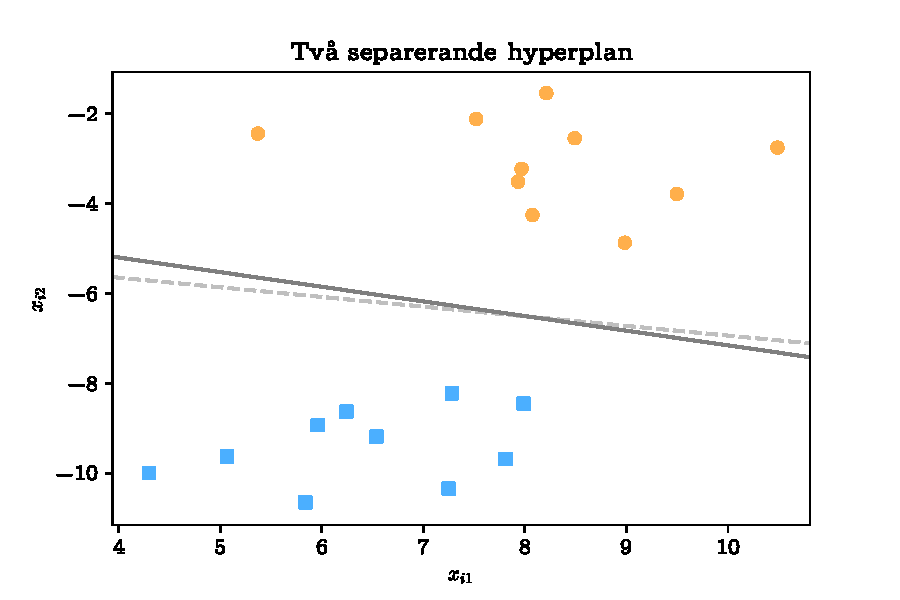
\includegraphics[width=0.8\linewidth, trim={0.5cm 2mm 0.5cm 6mm}, clip]{KandFigur1.pdf}
	\caption{\label{fig:separatinghyperplane}20 datapunkter med två separerande hyperplan (linjer) där klassen $y_i=1$ framställs som blå fyrkanter och klassen $y_i=-1$ som orangea cirklar.}
\end{figure}
\end{frame}

\begin{frame}
\frametitle{Stödvektormaskiner}
\framesubtitle{Enkel linjär klassificerare, optimalt separerande hyperplan}
Tanken är att man vill hitta ett hyperplan sådant att:
\begin{itemize}
	\item alla observationer klassificeras rätt och,
	\item hyperplanet samtidigt maximerar det kortaste avståndet från hyperplanet till det närmsta observationsparet.
\end{itemize}

Matematiskt kan man uttrycka problemet som följande optimeringsproblem
\begin{equation*}\label{opt:optimalmargin1}
\begin{aligned}
\operatornamewithlimits{max}_{\widehat{\bfbeta}, \widehat{\beta}_0, \left\|\widehat{\bfbeta}\right\|_p=1}& & &C\\
\text{så att}& & &y_i\left(\inner{\bfx_i}{\widehat{\bfbeta}}_p+\widehat{\beta}_0\right)\geq C,\quad i=1,~\dots,~N
\end{aligned}
\end{equation*}
där $C$ kallas \emph{marginalen} och betecknar avståndet från hyperplanet till de närmaste observationerna.
\end{frame}

\begin{frame}
\frametitle{Stödvektormaskiner}
\framesubtitle{Optimalt separerande hyperplan}
Transformera optimeringsproblemet
\begin{equation*}
\begin{aligned}
\operatornamewithlimits{max}_{\widehat{\bfbeta}, \widehat{\beta}_0, \left\|\widehat{\bfbeta}\right\|_p=1}& & &C\\
\text{så att}& & &y_i\left(\inner{\bfx_i}{\widehat{\bfbeta}}_p+\widehat{\beta}_0\right)\geq C,\quad i=1,~\dots,~N,
\end{aligned}
\end{equation*}
genom att välja $C=\frac{1}{\left\|\bfbeta
	\right\|_p}$ och kvadrera objektfunktionen, då fås optimeringsproblemet
	\begin{equation*}
	\begin{aligned}
	\operatornamewithlimits{min}_{\bfbeta, \beta_0} & & &\frac{1}{2}\left\|\bfbeta
	\right\|_p^2\\
	\text{så att} & & &y_i\left(\inner{\bfx_i}{\bfbeta}_p+\beta_0\right)\geq 1,\quad i=1,~\dots,~N.
	\end{aligned}
	\end{equation*}
\end{frame}

\begin{frame}
\frametitle{Stödvektormaskiner}
\framesubtitle{Lagrangeproblem}
Optimeringsproblemet löses genom Lagrangefunktionen som ges av
\begin{equation*}\label{eq:primallagrange}
L_P=\frac{1}{2}\inner{\bfbeta}{\bfbeta}_p - \sum_{i=1}^{N} \lambda_i\left(y_i \left(\inner{\bfx_i}{\bfbeta}_p + \beta_0\right)-1\right)
\end{equation*}
som ska minimeras med avseende på $\bfbeta$ och $\beta_0$. Efter differentiering och insättning av nollpunkterna i $L_P$ fås den duala Lagrangefunktionen
\begin{equation*}
L_D= -\frac{1}{2} \sum_{i=1}^{N} \sum_{j=1}^{N} \lambda_i \lambda_j y_i y_j \inner{\mathbf{x}_i}{\mathbf{x}_j}_p + \sum_{i=1}^{N} \lambda_i
\end{equation*}
som ska maximeras med avseende på $\lambda_i,~i=1,~\dots,~N,$ och kravet \begin{equation*}
\lambda_i\geq 0,\quad i=1,~\dots,~N.
\end{equation*} 
\end{frame}

\begin{frame}
\frametitle{Stödvektormaskiner}
\framesubtitle{Karush-Kuhn-Tucker}
Då måste den optimala lösningen $\bfbeta^*, \beta^*, \lambda_i^*$ uppfylla följande villkor:
\begin{align}
\frac{\partial L_P}{\partial \bfbeta}&\text{ ger }&\bfbeta^* &= \sum_{i=1}^{N} \lambda_i^* y_i \mathbf{x}_i,\label{eq:krav1}\\
\frac{\partial L_P}{\partial \beta}&\text{ ger }&0 &= \sum_{i=1}^{N} \lambda_i^* y_i,\label{eq:krav2}
\intertext{från differentieringen av $L_P$ och}
&& \lambda_i^*&\geq 0,\quad i=1, \dots, N,\label{eq:krav3}\\
&& \lambda_i^*\left( y_i\left( \inner{\bfx}{\bfbeta^*}_p + \beta^*_0 \right) -1 \right) &= 0,\quad i=1, \dots, N\label{eq:krav4}.
\end{align}
\end{frame}

\begin{frame}
\frametitle{Stödvektormaskiner}
\framesubtitle{Karaktärisering av lösningen}
%	Kraven (\ref{eq:krav1}) till (\ref{eq:krav4}) säger något om hurudan den optimala lösningen $\left(\bfbeta^*, \beta^*_0, \lambda_1^*, \dots, \lambda_N^*\right)$ måste vara:
\begin{itemize}
	\item Krav (\ref{eq:krav1}) säger att vektorn $\bfbeta^*$ är en linjär kombination av vektorerna $\mathbf{x}_i,~i=1,~\dots,~N$.
	\item Ifall $\lambda^*_i > 0$ så ger krav (\ref{eq:krav4}) att $y_i\left(\inner{\bfx_i}{\bfbeta^*}_p+\beta^*_0\right) = 1$. Punkten $\mathbf{x}_i$ är med andra ord en av punkterna som ligger närmast det separerande hyperplanet.
	\item Ifall $y_i\left(\inner{\bfx_i}{\bfbeta^*}_p + \beta^*_0\right) > 1$ så är $\lambda^*_i = 0$ och punkten $\mathbf{x}_i$ är inte en av punkterna som ligger närmast det separerande hyperplanet.
	\item Parametern $\beta^*_0$ kan bestämmas genom att man utnyttjar relationen $y_i\left(\inner{\bfx_i}{\bfbeta^*}_p + \beta^*_0\right) = 1$ för någon av punkterna där $\lambda^*_i > 0$.
\end{itemize}
Baserat på de tre tidigare slutsatserna kan man dra slutsatsen att $\bfbeta^*$ är en linjär kombination av endast de punkter $\mathbf{x}_{i}$ som ligger på randen av marginalen. En punkt som ligger på randen av marginalen kallas \emph{stödvektor}.
\end{frame}

\begin{frame}
\frametitle{Stödvektormaskiner}
\framesubtitle{Oseparabla problem}
Ifall ett optimeringsproblems krav gör det olösbart kan man tillåta lösningar som strider mot kraven och samtidigt försöka reglera hur långt från de ursprungliga kraven man tillåter lösningar. I praktiken åstadkoms detta med hjälp av \emph{slackvariabler} och lösningarna blir (separerande) \emph{hyperplan med mjuka marginaler}.

För optimalt separerande hyperplan finns bara kraven
\begin{equation*}
	y_i\left(\inner{\bfx_i}{\widehat{\bfbeta}}_p+\widehat{\beta}_0\right) \geq C, \qquad i=1,~\dots,~N
\end{equation*}
det vill säga kravet att observationsparen är linjärt separabla.
\end{frame}

\begin{frame}
\frametitle{Stödvektormaskiner}
\framesubtitle{Slackvariabler}
	För det ursprungliga optimeringsproblemet finns två naturliga sätt att ändra på kraven, endera låter man
	\begin{align}
	y_i\left(\inner{\bfx_i}{\widehat{\bfbeta}}_p+\widehat{\beta}_0\right) &\geq C-s_i,\label{eq:softändring1}\\
	\intertext{eller}
	y_i\left(\inner{\bfx_i}{\widehat{\bfbeta}}_p+\widehat{\beta}_0\right) &\geq C\left(1-s_i\right),\label{eq:softändring2}
	\end{align}
	där slackvariablerna $s_i\in\mathbb{R}$ är nedåt begränsade av noll samt uppåt begränsade så att summan av alla slackvariabler blir mindre än någon konstant $K$, det vill säga \begin{equation*}
	\begin{aligned}
	s_i&\geq0,\qquad i=1,~\dots,~N,\\
	\sum_{i=1}^{N}s_i&\leq K.
	\end{aligned}
	\end{equation*}
\end{frame}

\begin{frame}
\frametitle{Stödvektormaskiner}
\framesubtitle{Separerande hyperplan med mjuka marginaler}
För hyperplan med mjuka marginaler blir det ursprungliga optimeringsproblemet:
\begin{equation*}\label{opt:softmargin}
\begin{aligned}
\operatornamewithlimits{max}_{\widehat{\bfbeta}, \widehat{\beta}_0, \left\|\widehat{\bfbeta}
	\right\|_p=1}& & &C\\
\text{så att}& & &y_i\left(\inner{\bfx_i}{\widehat{\bfbeta}}_p+\widehat{\beta}_0\right)\geq C\left(1-s_i\right),\quad i=1,~\dots,~N,\\
& & &s_i\geq0,\quad i=1,~\dots,~N,\\
& & &\sum_{i=1}^{N}s_i \leq K.
\end{aligned}
\end{equation*}
\end{frame}

\begin{frame}
\frametitle{Stödvektormaskiner}
\framesubtitle{Separerande hyperplan med mjuka marginaler}
Optimeringsproblemet på föregående sida kan arbetas om till följande optimeringsproblem:
\begin{equation*}
\begin{aligned}
\operatornamewithlimits{min}_{\bfbeta, \beta_0} & & &\frac{1}{2}\left\|\bfbeta
\right\|_p^2\\
\text{så att} & & &y_i\left(\inner{\bfx_i}{\bfbeta}_p+\beta_0\right)\geq 1 - s_i,\quad i=1,~\dots,~N,\\
& & &s_i\geq0,\quad i=1,~\dots,~N,\\
& & &\sum_{i=1}^{N} s_i \leq K.
\end{aligned}
\end{equation*}

\end{frame}

\begin{frame}
\frametitle{Stödvektormaskiner}
\framesubtitle{Barriärmetoden}
Efter approximering av det sista kravet i objektfunktionen fås optimeringsproblemet:
\begin{equation*}\label{eq:softpenalty1}
\begin{aligned}
\operatornamewithlimits{min}_{\bfbeta, \beta_0} & & &\frac{1}{2}\left\|\bfbeta
\right\|_p^2 + \gamma\sum_{i=1}^{N} s_i\\
\text{så att} & & &y_i\left(\inner{\bfx_i}{\bfbeta}_p+\beta_0\right)\geq 1 - s_i,\quad i=1,~\dots,~N,\\
& & &s_i\geq0,\quad i=1,~\dots,~N,
\end{aligned}
\end{equation*}
som alltid är lösbart och kan lösas med Lagrangemultiplikatorer.
\end{frame}

\begin{frame}
\frametitle{Stödvektormaskiner}
\framesubtitle{Lagrangemultiplikatorer}
Den primala Lagrangefunktionen ges av
\begin{gather*}
L_P = \frac{1}{2}\inner{\bfbeta}{\bfbeta}_p+\gamma\sum_{i=1}^{N}s_i - \sum_{i=1}^{N}\lambda_i\left(y_i\left(\inner{\bfx_i}{\bfbeta}_p + \beta_0\right)-\left(1-s_i\right)\right)\\-\sum_{i=1}^{N}\mu_is_i.
\end{gather*}
Efter samma manipulationer som tidigare fås den duala Lagrangefunktionen:
\begin{gather*}
L_D = \sum_{i=1}^{N}\lambda_i - \frac{1}{2}\sum_{i=1}^{N}\sum_{j=1}^{N}\lambda_i\lambda_jy_iy_j\inner{\bfx_i}{\bfx_j}_p
\end{gather*}
som ska maximeras med avseende på $\lambda_i$, med kraven $0\leq\lambda_i\leq\gamma$ och $\sum_{i=1}^{N}\lambda_iy_i=0$.
\end{frame}

\begin{frame}
\frametitle{Stödvektormaskiner}
\framesubtitle{Krav}
Dessutom fås följande krav:
\begin{align}
\label{eq:softkrav1}	\bfbeta^* &= \sum_{i=1}^{N} \lambda_i^*y_i\mathbf{x}_i, & &\\
\label{eq:softkrav2}	0 &= \sum_{i=1}^{N} \lambda^*_iy_i, & &\\
\label{eq:softkrav3}	\lambda^*_i &= \gamma - \mu^*_i \quad& &i = 1,~\dots,~N,\\
\label{eq:softkrav4}	\lambda^*_i,~\mu^*_i,~s_i&\geq0,\quad& &i = 1,~\dots,~N.
\end{align}
\end{frame}

\begin{frame}
\frametitle{Stödvektormaskiner}
\framesubtitle{Karush-Kuhn-Tucker villkor}
Och följande krav
\begin{align}
\label{eq:softkrav7}	\lambda^*_i\left( y_i\left(\inner{\bfx_i}{\bfbeta^*}_p + \beta^*_0\right) - \left(1-s^*_i\right)\right) &= 0, \quad & &i = 1,~\dots,~N,\\
\label{eq:softkrav8}	\mu^*_is^*_i&=0, \quad & &i = 1,~\dots,~N,\\
\label{eq:softkrav9}	y_i\left(\inner{\bfx_i}{\bfbeta^*}_p+\beta^*_0\right)-\left(1-s^*_i\right) &\geq 0, \quad & &i = 1,~\dots,~N.
\end{align}
\end{frame}

\begin{frame}
\frametitle{Stödvektormaskiner}
\framesubtitle{Karaktärisering av lösningen}
	Precis som för algoritmen med optimala separerande hyperplan kan man karaktärisera lösningen för hyperplan med mjuka marginaler med hjälp av kraven (\ref{eq:softkrav1}) till (\ref{eq:softkrav9}).
	\begin{itemize}
		\item Krav (\ref{eq:softkrav1}) och (\ref{eq:softkrav7}) ger att den optimala lösningen $\bfbeta^*$ ges som den linjära kombinationen
		$\bfbeta^* = \sum_{i=1}^{N}\lambda_i^*y_i\mathbf{x}_i,$
		av punkter $\mathbf{x}_i$ på eller i marginalen. För punkterna på eller i marginalen gäller att $\lambda^*_i>0$, de kallas \emph{stödvektorer} eftersom de är de enda punkterna som behövs för att representera $\bfbeta^*$.
		\item För stödvektorer ($\lambda^*_i>0$) som ligger på marginalen ($s_i^*=0$) ger kraven (\ref{eq:softkrav3}) och (\ref{eq:softkrav8}) att $0<\lambda_i^*<\gamma$.
		\item För de resterande stödvektorerna ($\lambda_i^*>0$) gäller $\lambda_i^*=\gamma$.
		\item Vilken som helst av punkterna på marginalen ($\lambda^*_i>0,~s^*_i=0$) kan användas för att lösa för $\beta_0^*$.
	\end{itemize}
\end{frame}

\begin{frame}
\frametitle{Stödvektormaskiner}
\framesubtitle{Exempel}
\begin{figure}[h]
	\centering
	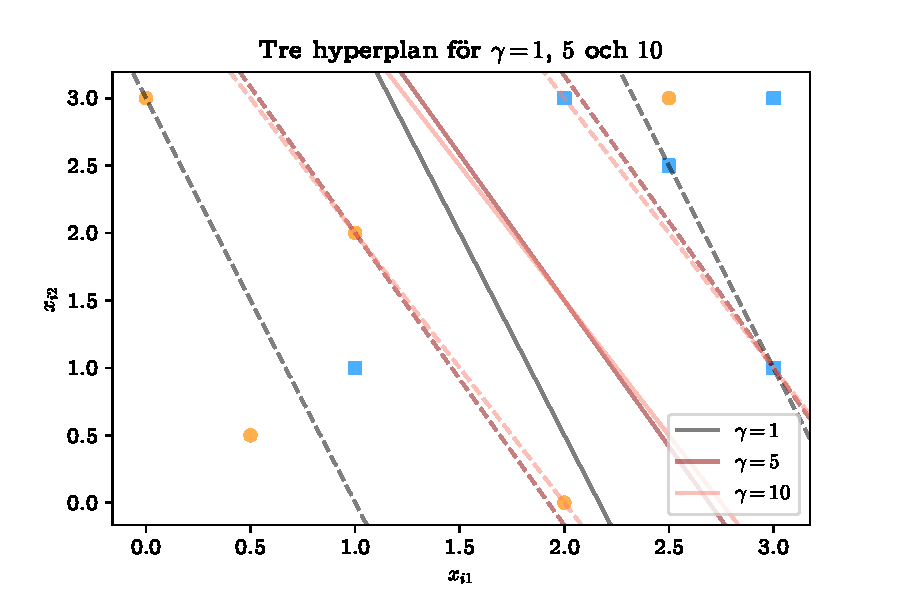
\includegraphics[width=0.8\linewidth, trim={0.5cm 2mm 0.5cm 6mm}, clip]{KandFigur2.pdf}
	\caption{\label{fig:mjukamarginaler}Löst exempel för linjärt oseparabelt data för 3 olika värden på $\gamma$. De streckade linjerna är marginalernas ränder.}
\end{figure}
\end{frame}

\begin{frame}
\frametitle{Stödvektormaskiner}
\framesubtitle{Exempel}
\begin{figure}[h]
	\centering
	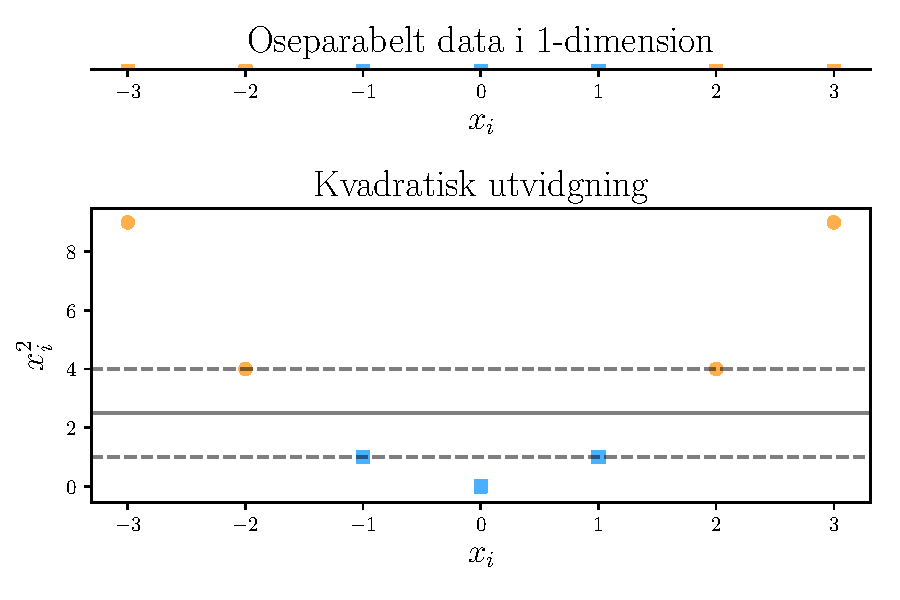
\includegraphics[width=0.8\linewidth, trim={0.5cm 4mm -5mm 4mm}, clip]{KandFigur3.pdf}
	\caption{\label{fig:kvadratisk}En lösning med optimala separerande hyperplan och kvadratisk utvidgning där endast hyperplan med mjuka marginaler inte hade fungerat.}
\end{figure}
\end{frame}

\begin{frame}
\frametitle{Stödvektormaskiner}
\framesubtitle{Exempel}
Klart är att observationsparen är linjärt oseparabla men nu kan inte heller separerande hyperplan med mjuka marginaler ge vettiga lösningar. Istället kan man lägga till en dimension och definiera att $\mathbf{x}_i\in\mathbb{R}^2$ och $\mathbf{x}_{i2} = \mathbf{x}_{i1}^2$.
Då får man situationen som illustreras nederst i föregående figur och observationsparen är nu linjärt separabla. Det optimala separerande hyperplanet bestämdes med hjälp av \texttt{sklearn}:s metod \texttt{SVC} med \texttt{kernel='linear'} och \texttt{C=1000}.

Moralen är att hyperplan med mjuka marginaler inte alltid räcker till utan flera verktyg behövs. Ett sådant verktyg är olinjära utvidgningar av det ursprungliga rummet $\mathbf{x}_i\in \mathbb{R}^p$ till ett större rum där det kan vara enklare att hitta vettiga klassificeringsregler.
\end{frame}

\begin{frame}
\frametitle{Reproducerande kärnor}
\framesubtitle{Fortsättning på exemplet}
Betrakta funktionen $\phi:\left[\bfx\right]\longmapsto \left[\bfx^2,\sqrt{2}\bfx, 1\right]^\intercal$ där $\bfx\in\mathbb{R}$, denna funktion motsvarar den olinjära utvidgningen i föregående. Följande inreprodukt mellan två observationer $\mathbf{x}_1$ och $\mathbf{x}_2$ ska beräknas:
\begin{align*}
\left\langle \phi\left(\mathbf{x}_1\right), \phi\left(\mathbf{x}_2\right) \right\rangle_3 &= \bfx_1^2\bfx_2^2 + 2\bfx_1\bfx_2 + 1\\
&= \langle \bfx_1, \bfx_2 \rangle_1^2 + 2\langle \bfx_1, \bfx_2 \rangle_1 + 1\\
&= \left(\langle\bfx_1, \bfx_2 \rangle_1 + 1\right)^2 = k\left(\bfx_1, \bfx_2\right)
\end{align*}
där $\langle \cdot, \cdot \rangle_p$ är den vanliga inreprodukten i $\mathbb{R}^p$.
\end{frame}

\begin{frame}
\frametitle{Reproducerande kärnor}
\framesubtitle{Fortsättning på exemplet}
	Man byter alltså ut inreprodukten $\inner{\phi\left(\bfx_i\right)}{\phi\left(\bfx_j\right)}_3$ mot funktionen $k\left(\bfx_i, \bfx_j\right)=\left(\langle\bfx_1, \bfx_2 \rangle_1 + 1\right)^2$ när man löser optimeringsproblemet. I det här fallet gör man inga större besparingar när man räknar ut matrisen $\mathbf{K}_{ij}=\inner{\bfx_i}{\bfx_j}$, eftersom inreprodukten $\inner{[\bfx_i^2, \bfx_i]^\intercal}{[\bfx_j^2, \bfx_j]^\intercal}_2$ endast kräver 3 operationer att beräkna, lika många som funktionen $k$. Ifall man hade använt femte gradens polynom hade funktionen $k\left(\bfx_i, \bfx_j\right)=\left(\langle\bfx_1, \bfx_2 \rangle_1 + 1\right)^5$ krävt mellan 3 och 5 operationer att beräkna (beroende på hur exponentiering är implementerat\footnote{Antalet operationer blir 3 ifall datorn kan räkna ut $a^5$ med en operation, annars är $a^5=a^2a^2a$ där man inte behöver räkna ut $a^2$ två gånger och antalet operationer blir 5.}) medan inreprodukten $\inner{\cdot}{\cdot}_4$ kräver 7 operationer att räkna.
	
	Man behöver dessutom inte räkna ut utvidgningen på förhand.
\end{frame}

\begin{frame}
\frametitle{Reproducerande kärnor}
\framesubtitle{Kärnor som inreprodukter}
\begin{defi}\label{def:kärna}
	Givet en funktion $\phi: \mathbb{R}^p \longmapsto \mathbb{R}^P$ definieras \emph{kärnan} $k$ som funktionen $k\left(\bfx, \bfy\right) = \langle \phi \left(\bfx\right), \phi\left(\bfy\right) \rangle_P$ där $\bfx, \bfy \in \mathbb{R}^p$ och $\langle \cdot, \cdot \rangle_P$ är den vanliga inreprodukten i $\mathbb{R}^P$.
	Vidare om man fixerar ett $\bfy\in\mathbb{R}^p$ så betecknar vi $\Phi_{\bfy}\left(\bfx\right) = k\left(\bfx, \bfy\right)$ där $\bfx\in\mathbb{R}^p$.
\end{defi}
Givet en mängd observationer $\bfx_i\in\mathbb{R},~i=1,~\dots,~N$, samt den polynomiella kärnan $k\left(\bfx, \bfy\right):=\left(\langle \bfx, \bfy \rangle_1 + 1\right)^2 = \left(\bfx\bfy\right)^{2} + 2\bfx\bfy + 1$, kan man definiera ett vektorrum av funktioner genom
\begin{equation*}
f\left(\bfx\right):=\sum_{i=1}^{N}\alpha_ik\left(\bfx, \bfx_i\right)\quad ,~\alpha_i\in\mathbb{R}.
\end{equation*}
Varje funktion $f\left(\bfx\right)$ är alltså en linjär kombination av funktionerna $\Phi_{\bfx_i}\left(\bfx\right)=k\left(\bfx,\bfx_i\right)$ där $\bfx_i,~i=1,~\dots,~N$ är fixerade.
\end{frame}

\begin{frame}
\frametitle{Reproducerande kärnor}
\framesubtitle{En till inreprodukt}
För en annan funktion $g\left(\bfx\right):=\sum_{j=1}^{m}\beta_jk\left(\bfx, \bfx_j\right)$ i samma vektorrum kan man definiera inreprodukten
\begin{equation*}\label{eq:polykärnaprodukt}
\langle f , g\rangle_k := \sum_{i=1}^{N}\sum_{j=1}^{N} \alpha_i \beta_j k\left(\bfx_i, \bfx_j\right).
\end{equation*}
I beviset för att detta är en inreprodukt stöder man sig på att funktionen $k$ är symmetrisk och positivt semidefinit (eftersom att kärnan är en inreprodukt).

Om man istället definierar en kärna på följande sätt borde beviset fortfarande fungera:
\begin{defi}
	En kärna är en symmetrisk positivt semidefinit funktion $k: X \times X \longmapsto \mathbb{R}$.
\end{defi}
\end{frame}

\begin{frame}
\frametitle{Reproducerande kärnor}
\framesubtitle{Reproducerande}
Betrakta funktionen $\Phi_{\bfx_l}(\bfx):=k\left(\bfx, \bfx_l\right)$, där $k\left(\bfx, \bfy\right)$ är en symmetrisk positivt semidefinit funktion.  Funktionen $\Phi_{\bfx_l}\!(\bfx)$ kan skrivas som $\sum_{j=1}^{N}\!\beta_jk\left(\bfx, \bfx_l\right)$ med $\beta_j=1$ om $j=l$, 0 annars, för att passa in i definitionen för inreprodukten $\inner{\cdot}{\cdot}_k$. För $\Phi_{\bfx_l}(\bfx)$ och en annan funktion $f\left(\bfx\right) = \sum_{i=1}^{N}\alpha_ik\left(\bfx, \bfx_i\right)$ gäller då att
\begin{equation*}
\langle \Phi_{\bfx_l}, f\rangle_k = \langle k\left(\cdot, \bfx_i\right), f\rangle_k = \sum_{j=1}^{N}\sum_{i=1}^{N}\beta_j\alpha_i k\left(\bfx_j, \bfx_i\right)
\end{equation*}
där $\beta_j = 0$ om $j\neq l$ och $1$ om $j=l$, det vill säga
\begin{equation*}\label{eq:reproducing1}
\langle \Phi_{\bfx_l}, f\rangle_k = \sum_{i=1}^{N}\alpha_i k\left(\bfx_l, \bfx_i\right) = f\left(\bfx_l\right).
\end{equation*}
Tolkningen är att inreprodukten mellan en funktion $f$ och $k\left(\cdot, \bfx_i\right)$ är samma sak som evaluering av funktionen $f$ i punkten $\bfx_i$ men $\bfx_i$ måste vara en av de punkterna som man byggde upp inreprodukten av.

\end{frame}

\begin{frame}
\frametitle{Reproducerande kärnor}
\framesubtitle{Reproducerande}
Speciellt för en annan funktion $\Phi_{\bfx_h}(\bfx):=k\left(\bfx, \bfx_h\right)$ fås att
\begin{equation*}
\langle \Phi_{\bfx_l}, \Phi_{\bfx_h} \rangle_k = \sum_{i=1}^{N}\sum_{j=1}^{N}\alpha_i\beta_jk\left(\bfx_i, \bfx_j\right)
\end{equation*}
där $\alpha_i=\beta_j=1$ endast om $i=l$ och $j=h$, $\alpha_i=\beta_j=0$ annars. Då fås
\begin{equation*}\label{eq:reproducing2}
\begin{aligned}
\langle \Phi_{\bfx_l}, \Phi_{\bfx_h} \rangle_k &= \inner{k\left(\cdot, \bfx_l\right)}{k\left(\cdot, \bfx_h\right)}_k\\ &= \alpha_l\beta_hk\left(\bfx_l, \bfx_h\right)\\&= k\left(\bfx_l, \bfx_h\right).
\end{aligned}
\end{equation*}
Här är tolkningen att även om $k\left(\bfx_l, \bfx_h\right)$ inte är definierad genom en inreprodukt så kan $k$ tolkas som en inreprodukt i något (olinjärt) rum. De här två egenskaperna är orsaken till att man pratar om \emph{reproducerande} kärnor, den första ekvationen brukar också ibland användas som definitionen på en reproducerande kärna.
\end{frame}

\begin{frame}
\frametitle{Reproducerande kärnor}
\framesubtitle{Inreprodukt i något rum}
Med andra ord borde man givet en symmetrisk positivt semidefinit funktion $k$ kunna skriva den som en inreprodukt i något rum.
	Låt $\bfx_i,~\bfx_j\in\mathbb{R}$ och betrakta funktionen
\begin{align*}
k\left(\bfx_i, \bfx_j\right)&=e^{-\frac{\left\| \bfx_i-\bfx_j\right\|_1^2}{2\sigma^2}}\\&=e^{-\frac{\inner{\bfx_i-\bfx_j}{\bfx_i-\bfx_j}_1}{2\sigma^2}}\\
&=e^{-\frac{\bfx_i^2+\bfx_j^2-2\bfx_i\bfx_j}{2\sigma^2}}\\&=e^{-\frac{\bfx_i^2+\bfx_j^2}{2\sigma^2}}\cdot e^{\frac{2\bfx_i\bfx_j}{2\sigma^2}}\\
&= e^{-\left(\frac{\bfx_i}{\sqrt{2}\sigma}\right)^2}\cdot e^{-\left(\frac{\bfx_j}{\sqrt{2}\sigma}\right)^2}\cdot e^{\frac{\bfx_i\bfx_j}{\sigma^2}}.
\end{align*}

\end{frame}

\begin{frame}
\frametitle{Reproducerande kärnor}
\framesubtitle{Fortsättning på exemplet}
Genom Taylorutvecklingen för $e^{z}$ fås
\begin{align*}
k\left(\bfx_i, \bfx_j\right)&= e^{-\left(\frac{\bfx_i}{\sqrt{2}\sigma}\right)^2}\cdot e^{-\left(\frac{\bfx_j}{\sqrt{2}\sigma}\right)^2}\cdot \sum_{n=0}^{\infty}\frac{\bfx_i^n\bfx_j^n}{n!}\\
&= \sum_{n=0}^{\infty} \left(\frac{e^{-\left(\frac{\bfx_i}{\sqrt{2}\sigma}\right)^2} \bfx_i^n}{\sqrt{n!}}\right)\left(\frac{e^{-\left(\frac{\bfx_j}{\sqrt{2}\sigma}\right)^2} \bfx_j^n}{\sqrt{n!}}\right)\\
&= \inner{\phi\left(\bfx_i\right)}{\phi\left(\bfx_j\right)}_{\ell^2}
\end{align*}
där $\inner{\bfx}{\bfy}_{\ell^2}$ är inreprodukten given av summan $\sum_{h=1}^{\infty}\bfx_h\bfy_h$ om den är ändlig. Här betecknar $\bfx_h$ och $\bfy_h$ de $h$:te komponenterna av de oändligtdimensionella vektorerna $\bfx$ och $\bfy$. Summan konvergerar om $\bfx$ och $\bfy$ tillhör Hilbertrummet $\ell^2$ det vill säga rummet av alla följder $\bfx$ för vilka summan $\sum_{h=1}^{\infty}\bfx_h^2=\inner{\bfx}{\bfx}_{\ell^2}=\left\|\bfx\right\|_{\ell^2}^2$ är ändlig.
\end{frame}

\begin{frame}
\frametitle{Reproducerande kärnor}
\framesubtitle{Fortsättning på exemplet}
Kärnan $k\left(\bfx, \bfy\right)=e^{-\frac{\left\| \bfx-\bfy\right\|^2}{2\sigma^2}}$ kan med andra ord skrivas som inreprodukten $\inner{\phi\left(\bfx\right)}{\phi\left(\bfy\right)}_{\ell^2}$ i rummet som ges av utvidgningen
\begin{equation*}
\phi\left(\bfx\right)=\left[\frac{e^{-\left(\frac{\bfx}{\sqrt{2}\sigma}\right)^2} \bfx^0}{\sqrt{0!}}, \frac{e^{-\left(\frac{\bfx}{\sqrt{2}\sigma}\right)^2} \bfx^1}{\sqrt{1!}}, \frac{e^{-\left(\frac{\bfx}{\sqrt{2}\sigma}\right)^2} \bfx^2}{\sqrt{2!}}, \dots\right]^\intercal.
\end{equation*}

Implikationen är att motsvarande olinjära transformation skulle ge ett oändligtdimensionellt rum att jobba med om man gör transformationen direkt medan man genom kärnan $k$ implicit kan jobba i ett oändligtdimensionellt rum, något som inte hade varit möjligt om man försökte operera med vanliga inreprodukter på det utvidgade rummet.
\end{frame}

\end{document}
